%%%%%%%%%%%%%%%%%%%%%%%%%%%%%%%%%%%%%%%%%%%%%%%%%%%%%%
\section{Evaluation}
\label{sec:eval}
% \ugh{ASSIGNED TO: Amanda}\\
%%%%%%%%%%%%%%%%%%%%%%%%%%%%%%%%%%%%%%%%%%%%%%%%%%%%%%
% \ac{Outline:
% \begin{itemize}
%     \item Quick explanation as to what this eval shows
%     \item Explain the experiment setup. This should discuss mininet and how the programs measure things and where
%     \item Explain the remote paging latency
%     \item Explain the RDMA speed up compared to disk
% \end{itemize}}
% Our proof of concept shows that IPv6 addressed memory is possible, but one critical aspect that must be evaluated is the overhead incurred by remote paging. 
We evaluate our implementation in two ways. First, we look at the simulated speed up with a directory service switch to determine the overhead improvement our design brings. Next, we consider how the overhead compares to disk access if the communication used is RDMA. 


\subsection{Experimental Setup}
As mentioned in Section \ref{sec:implementation}, we used Mininet to simulate the network and switch for our tests. In our evaluation, we have three hosts, three servers, three NDP proxies, one switch, and one controller. Mininet was run on a machine with an Intel(R) Core(TM)2 Quad CPU Q9400 @ 2.66GHz, 4 GB of memory, and the mininet configuration reached a peak bandwidth of about 800 Mbits/sec. Each experiment was measured in nanoseconds, when the median latency and 95th percentile were calculated, the latencies were then converted into $\mu$s.

As mentioned before, this implementation uses a static switch configuration (learning switch). Although this makes our performance numbers not entirely representative of our proposed design, it does provide a good indication as to how the system will perform once it is fully built. 

% \ac{Would this be better in the implementation section? Is it even necessary?} We measure latency using the \texttt{timespec} struct in C and \texttt{clock\_gettime$\left(\text{CLOCK\_MONOTONIC,...}\right)$}. Our latency measurements are taken in nanoseconds and, when analyzed, they are converted into $\mu$s. 

\subsection{Remote Paging Latency}
% \ac{Outline:
% \begin{itemize}
%     \item Reiterate main goal of proof of concept: to show feasibility of IPv6 addressing
%     \item Claimed improvement --> reduced overhead due to one less RTT
%     \item But how much will that actually improve things?
%     \item Explain experiment setup (i.e., 1500 pages, userfaultfd program, not actually doing a remote write, etc.)
%     \item Discuss total latency comparison first
%     \item Discuss read and write breakdown, highlight how the RTTs are the worst part of the latency, therefore removing one makes a huge impact. 
%     \item Segway into RDMA discussion
% \end{itemize}
% }
One of the main benefits of moving the management into the switch is the improved performance. This improved performance comes from reducing a roundtrip time (RTT) to the directory service. But this assumes that the RTT to a directory service incurs enough cost to affect the overall latency. To explore this, we simulated three scenarios: 1) shared memory system with a centralized directory service, 2) shared memory system with a directory service in the switch, and 3) a normal system disk access. We include the disk access in our measurements to provide a baseline for comparisons. We do not claim that we currently outperform a disk access, although our performance numbers point to the ability to do so with proper optimizations.

The shared memory system with a centralized directory service (Remote w/ DS) is simulated by querying the server for the IPv6 address of a piece of memory it requires to access. The server will then respond with an IPv6-compliant pointer for the client to use in a READ request. The shared memory with a directory service in the switch (Remote w/o DS) stores the IPv6-compliant pointer when allocating the memory, thus allowing it to skip the step of asking a directory service which machine to send its pointer to. This is not our exact design, as we would have a rule in the switch which recognizes which machine to send this pointer. It will be similar in overhead cost because it does not query the directory service. 
% A decentralized shared memory platform would behave similarly, but only because it requires communication when memory moves, not on every access. Since we do not have a controller implemented for our solution, we do not compare to the decentralized shared memory, we save this for future work. 
The normal system disk access (Local) reads a dummy file from disk and loads it into memory. 

We ran each program with 1,500 pages, where it accesses each page once. We record the latency at multiple points of the execution path to determine where each program spends most of its time as well as the total latency. We then graph the median of these latencies with the 95th percentile error bars. The total latency is shown in Figure \ref{fig:total_latency} and appears as expected. The Remote w/ DS performs the worst and the disk access performs the best. We expected the disk access to perform the best because we did not optimize our proof of concept to use RDMA, therefore avoiding the server CPU. We discuss the implications of using RDMA in the next section.

\begin{figure}[t]
    \centering
    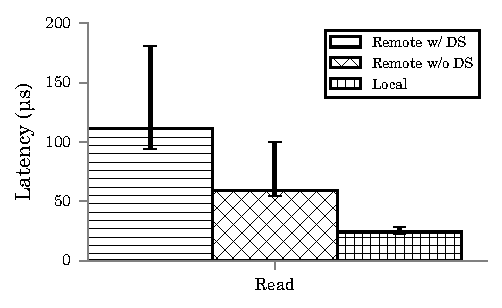
\includegraphics{Graphs/Latency_Total_Comparison.pdf}
    \caption{A comparison of the total latency per page fault of reads under three conditions: remote read with a directory service call, remote read without a directory service call, and accessing local disk. This is the median latency over 1,500 accesses of different pages with 95th percentile error bars.}
    \label{fig:total_latency}
\end{figure}

We breakdown the total latency into five categories: enter handler, exit handler, access DS (directory service), get data, and other. Enter handler is the amount of time it takes from the application level access of a page which faults till the handler receives the event notification. Exit handler is the time it takes after the handler finishes its work till the application is no longer blocked. Access DS is the amount of time the handler spent querying the directory service for the machine to send the request to. Get data is the amount of time the handler spends getting the data from the remote host or disk. 

The interesting part of the latency breakdown, Figure \ref{fig:read_breakdown}, is how much time the Access DS and Get data take compared to the other operations, they take approximately 9x longer. Based on that, it's obvious that reducing the execution path to one RTT instead of two is desirable. The reason the RTTs are drastically slower is the fact that we perform all communications over UDP on Ethernet. If these operations were done with RDMA, there should be a more significant speed up.

\begin{figure}[t]
    \centering
    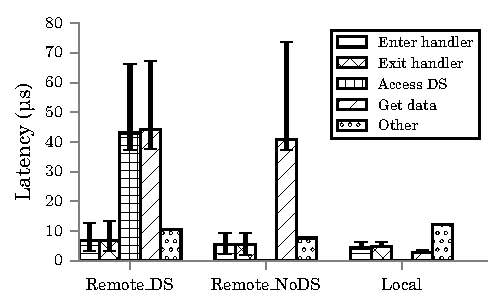
\includegraphics{Graphs/Latency_Breakdown_Read.pdf}
    \caption{A breakdown of the latency cost for a read under three conditions: remote read with a directory service call, remote read without a directory service call, and accessing local disk. This is the median latency over 1,500 accesses of different pages with 95th percentile error bars.}
    \label{fig:read_breakdown}
\end{figure}

% \begin{figure}[t]
%     \centering
%     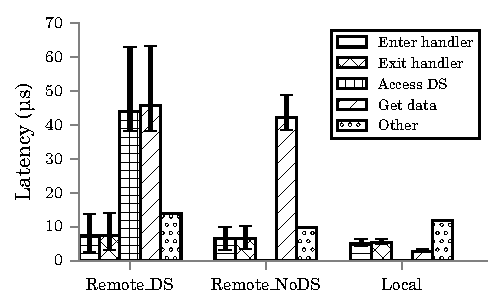
\includegraphics{Graphs/Latency_Breakdown_Write.pdf}
%     \caption{A breakdown of the latency cost for a write under three conditions: remote write with a directory service call, remote read without a directory service call, and accessing local disk. This is the median latency over 1,500 accesses of different pages with 95th percentile error bars.}
%     \label{fig:write_breakdown}
% \end{figure}

\subsection{Potential Gains of RDMA}
% \ac{Need better subsection title.}
% Outline:
% \begin{itemize}
%     \item As seen above, there is something to gain from removing the directory service, but still much higher latency than disk.
%     \item Well, original design uses RDMA, so how much will it improve things?
% \end{itemize}
% }
Most modern shared or remote memory systems leverage RDMA. Due to time constraints we could not leverage it for our proof of concept, but we still consider it in our performance evaluation. In our latency breakdown, we found that the RTT costs approximately 9x more than any of the other operations, which indicates that moving the directory service into the switch is very beneficial. But, we performed all communication in a non-optimal way, therefore we compare the amount of time it takes each remote operation with our communication method (UDP) and the equivalent RDMA method.

We have four operations, as stated in Section \ref{sec:overview}, CREATE, READ, UPDATE, DELETE. The RDMA equivalent for READ and UPDATE is RDMA read and RDMA write, respectively. CREATE and DELETE can be achieved using RDMA send/recv to issue commands to the remote server. According to experiments done by Ma et al. and Zhu et al., the approximate cost for an RDMA read or write operation is 3.4 $\mu$s and the approximate cost for an RDMA send/recv is 5.6 $\mu$s~\cite{Ma2016, Zhu2015}.\footnote{Reported latencies were one-way latencies for 2k and 4k pages. We doubled the reported latencies to make them roundtrip} We measured the latency of a small RDMA cluster using \texttt{qperf} to get one-way latencies for 4096 bytes. They mainly aligned with the numbers reported in \cite{Ma2016, Zhu2015}, so we use them in Table \ref{table:rdma_compare}.

As seen in Table \ref{table:rdma_compare}, using RDMA primitives instead of UDP improves the roundtrip time by 6x. Even with the improved communication latency, accessing a remote directory service incurs a high cost. In the worst case, it uses UDP and adds 45 $\mu$s, in the best case it uses RDMA primitives and adds 5.84 $\mu$s. It is still unnecessary overhead which can be mitigated by moving the directory service into the switch.

Another interesting observation of using RDMA, is that the theoretical latency would bring the total latency of our proposed solution into the same range as local disk. Our solution with the theoretical RDMA latency would cost approximately 22.116 $\mu$s, whereas the local disk latency is 24.304 $\mu$s.

\begin{table}[t]
    \begin{tabular}{ | l | l | l | l | }
        \hline
        & UDP ($\mu$s) & RDMA ($\mu$s) & Speed-up (x) \\ 
        \hline\hline
        Create & 34.919 & 5.84 & 5.979\\
        \hline
        Read & 33.732 & 5.92 & 5.698\\  
        \hline
        Update & 34.151 & 5.96 & 5.730\\
        \hline
        Delete & 32.963 & 5.84 & 5.644\\
        \hline
    \end{tabular}
    \caption{Comparison of our communication operations vs. their RDMA equivalent. For READ and UPDATE, the equivalents are RDMA read and write. For CREATE and DELETE, the equivalent is RDMA send/recv. Our latency medians were gathered over 1,500 runs of each operation. The RDMA measurements were gathered using \texttt{qperf}.}
    \label{table:rdma_compare}
\end{table}


% \begin{figure}
%     \centering
%     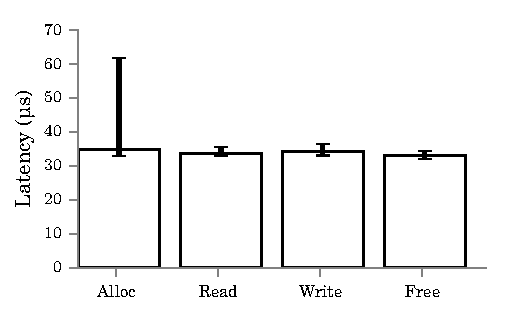
\includegraphics{Graphs/Microbenchmarks_Latency.pdf}
%     \caption{The median latency cost of each remote operation over 1,500 calls with 95th percentile error bars.}
%     \label{fig:micro_latency}
% \end{figure}

\subsection{Data Migration}
We attempted to perform data migration in our proof of concept system. Unfortunately, due to the NDP proxies required and the current network setup, data migration did not work. The switch was able to re-route the packets and the memory could easily be allocated at the same address on the new host server using \texttt{mmap()}, but the packets were getting dropped by the Linux network stack on the receiving server. This is because they were coming from an unknown address. Our system circumvents this issue by using the NDP proxies, but these do not work in the data migration case. Once we build a system which uses raw sockets and does not rely on NDP proxies, we will evaluate the data migration. We believe that data migration will work once the networking issues are fixed. 

\subsection{Observations}
While running our tests we made several interesting observations.

\subsubsection{NDP Table Exhaustion Attack}
\label{sec:silly_ndp}
As we increased the number of pointers to access we noticed our program continuously deadlocking around the 1000th to 1500th iteration. The packet of the client never reached its destination. However, neither server nor client showed signs of exhaustion and race conditions were unlikely due to the strictly sequential nature of the program. We initially suspected the switch to overload and drop packets, but the device forwarded correctly. The actual fault occurred on the client side. Although the \texttt{send()} system call of the program returned correctly without error, the packet was never forwarded to the interface. The cause of this issue was the NDP neighbor table on the client host. The client accidentally performed a NDP Table Exhaustion Attack~\cite{RFC3756} (see Figure \ref{lst:ndp_err}) on its own NDP neighbor table. The protocol generates a mapping for every unique IPv6 address to the destination interface. While the client allocates several thousand pointers, several thousand entries are created in the table. By default Ubuntu's NDP tables only have a size of around 4096 byte and the values expire slowly. The table is quickly exhausted and no entries can be created, which leads to a packet being quietly dropped and the program stalling. It seems that the only effective mitigation technique is to increase table size. NDP Neighbor tables do not seem offer netmask level matching nor is it possible explicitly specify a expiration time lower than 1 second. This is a crucial design flaw and further motivation to abolish NDP in our system. As we are moving towards raw socket messaging regardless, we are, as of this moment, not concerned about this problematic behavior.

\begin{figure}
\parbox[b][12px][t]{0.45\textwidth}{
 \footnotesize
 \texttt{[46768.440041] neighbour: ndisc\_cache: neighbor table overflow!}\\
 \texttt{[46770.564832]~neighbour: ndisc\_cache: neighbor table overflow!}\\
 \texttt{[46770.580728] neighbour: ndisc\_cache: neighbor table overflow!}
 } 
\caption{NDP table exhaustion error messages.}
\label{lst:ndp_err}
\end{figure}
\subsubsection{Mininet Performance Limits}
Initially we planned to test the rack-scale scalability of our system on Mininet. However, we faced limitations regarding the physical resources of our test machines. We conducted the tests on a Ubuntu 16.04 LTS machine with 12GB of RAM and a four-core i5 760 @ 2.80GHz processor. The first test involved launching 42 hosts, each running a client/server process as well as ndp-proxy daemon. Each client performed a 100 full iterations, but the test did not complete as several clients froze

In the second test, a single client performed a 1000 full iterations. The client also froze. 
A 42 unit Mininet cluster significantly stresses the CPU of the host system, thus it is unclear whether these results are due to Mininet's scalability constraints or design flaws in our system.
In addition, NDP seems to be a significant contributor to the load on the system. As every system maintains neighbor discovery, new pointers create solicitation storms across all nodes.
We plan to retry these tests after implementing raw socket messaging.

\subsubsection{Disk Access Latency} The reported disk access latency numbers (Local in Figure \ref{fig:total_latency}) are much lower than previously reported disk access latencies in literature. This is due to the file being accessed from the buffer cache instead of the disk every read. Since the page fault handler reads the same file, at the offset of 0, the file's content is most likely stored in the buffer cache instead of causing a disk seek every access. We plan to re-run the tests in future work with a larger file, random offsets, and buffer cache flushing to ensure that the file is read from disk every page fault.
% \fr{\\Does flushing the buffer cache not work?\\ https://unix.stackexchange.com/questions/87908/how-do-you-empty-the-buffers-and-cache-on-a-linux-system\\
% https://www.chrisnewland.com/clear-linux-buffers-cache-when-benchmarking-filesystem-337}
% \ac{It does, but I don't have the time to implement it. }